% Options for packages loaded elsewhere
\PassOptionsToPackage{unicode}{hyperref}
\PassOptionsToPackage{hyphens}{url}
\PassOptionsToPackage{dvipsnames,svgnames*,x11names*}{xcolor}
%
\documentclass[
  10pt,
]{article}
\usepackage{lmodern}
\usepackage{setspace}
\usepackage{amssymb,amsmath}
\usepackage{ifxetex,ifluatex}
\ifnum 0\ifxetex 1\fi\ifluatex 1\fi=0 % if pdftex
  \usepackage[T1]{fontenc}
  \usepackage[utf8]{inputenc}
  \usepackage{textcomp} % provide euro and other symbols
\else % if luatex or xetex
  \usepackage{unicode-math}
  \defaultfontfeatures{Scale=MatchLowercase}
  \defaultfontfeatures[\rmfamily]{Ligatures=TeX,Scale=1}
  \setmainfont[]{DejaVu Serif}
  \setmonofont[]{DejaVu Sans Mono}
\fi
% Use upquote if available, for straight quotes in verbatim environments
\IfFileExists{upquote.sty}{\usepackage{upquote}}{}
\IfFileExists{microtype.sty}{% use microtype if available
  \usepackage[]{microtype}
  \UseMicrotypeSet[protrusion]{basicmath} % disable protrusion for tt fonts
}{}
\makeatletter
\@ifundefined{KOMAClassName}{% if non-KOMA class
  \IfFileExists{parskip.sty}{%
    \usepackage{parskip}
  }{% else
    \setlength{\parindent}{0pt}
    \setlength{\parskip}{6pt plus 2pt minus 1pt}}
}{% if KOMA class
  \KOMAoptions{parskip=half}}
\makeatother
\usepackage{xcolor}
\IfFileExists{xurl.sty}{\usepackage{xurl}}{} % add URL line breaks if available
\IfFileExists{bookmark.sty}{\usepackage{bookmark}}{\usepackage{hyperref}}
\hypersetup{
  colorlinks=true,
  linkcolor=red,
  filecolor=red,
  citecolor=red,
  urlcolor=red,
  pdfcreator={LaTeX via pandoc}}
\urlstyle{same} % disable monospaced font for URLs
\usepackage[margin=1cm,top=1cm,bottom=1cm,left=1cm,right=1cm,includeheadfoot]{geometry}
\usepackage{listings}
\newcommand{\passthrough}[1]{#1}
\lstset{defaultdialect=[5.3]Lua}
\lstset{defaultdialect=[x86masm]Assembler}
\usepackage{graphicx}
\makeatletter
\def\maxwidth{\ifdim\Gin@nat@width>\linewidth\linewidth\else\Gin@nat@width\fi}
\def\maxheight{\ifdim\Gin@nat@height>\textheight\textheight\else\Gin@nat@height\fi}
\makeatother
% Scale images if necessary, so that they will not overflow the page
% margins by default, and it is still possible to overwrite the defaults
% using explicit options in \includegraphics[width, height, ...]{}
\setkeys{Gin}{width=\maxwidth,height=\maxheight,keepaspectratio}
% Set default figure placement to htbp
\makeatletter
\def\fps@figure{htbp}
\makeatother
\setlength{\emergencystretch}{3em} % prevent overfull lines
\providecommand{\tightlist}{%
  \setlength{\itemsep}{0pt}\setlength{\parskip}{0pt}}
\setcounter{secnumdepth}{3}
% Enable graphics inclusion and ensure figure numbering works
\usepackage{graphicx}
\renewcommand{\figurename}{Figure}

% Configure fonts for Unicode support with fallbacks
\usepackage{newunicodechar}
\newunicodechar{⁴}{\textsuperscript{4}}
\newunicodechar{₄}{\textsubscript{4}}

% Enhanced code block styling for better contrast and readability
\usepackage{fancyvrb}
\usepackage{xcolor}
\usepackage{listings}

% Define custom colors for code blocks
\definecolor{codebg}{RGB}{245, 245, 245}      % Light gray background
\definecolor{codeborder}{RGB}{200, 200, 200}  % Medium gray border
\definecolor{codefg}{RGB}{50, 50, 50}         % Dark gray text

% Configure Verbatim environment for inline code
\DefineVerbatimEnvironment{Verbatim}{Verbatim}{%
    fontsize=\small,
    frame=single,
    framerule=0.5pt,
    framesep=3pt,
    rulecolor=\color{codeborder},
    bgcolor=\color{codebg},
    fgcolor=\color{codefg}
}

% Configure code block styling
\DefineVerbatimEnvironment{Highlighting}{Verbatim}{%
    fontsize=\footnotesize,
    frame=single,
    framerule=0.5pt,
    framesep=5pt,
    rulecolor=\color{codeborder},
    bgcolor=\color{codebg},
    fgcolor=\color{codefg}
}

% Style inline code with \texttt
\renewcommand{\texttt}[1]{%
    \colorbox{codebg}{\color{codefg}\ttfamily #1}%
}

% Configure listings package for code blocks
\lstset{
    backgroundcolor=\color{codebg},
    basicstyle=\footnotesize\ttfamily\color{codefg},
    breakatwhitespace=false,
    breaklines=true,
    captionpos=b,
    commentstyle=\color{codefg},
    deletekeywords={...},
    escapeinside={\%*}{*)},
    extendedchars=true,
    frame=single,
    framerule=0.5pt,
    framesep=5pt,
    keepspaces=true,
    keywordstyle=\color{codefg},
    language=Python,
    morekeywords={*,...},
    numbers=left,
    numbersep=5pt,
    numberstyle=\tiny\color{codefg},
    rulecolor=\color{codeborder},
    showspaces=false,
    showstringspaces=false,
    showtabs=false,
    stepnumber=1,
    stringstyle=\color{codefg},
    tabsize=2,
    title=\lstname
}

% Override any Pandoc default lstset configurations
\AtBeginDocument{
    \lstset{
        backgroundcolor=\color{codebg},
        basicstyle=\footnotesize\ttfamily\color{codefg},
        frame=single,
        framerule=0.5pt,
        framesep=5pt,
        rulecolor=\color{codeborder},
        numbers=left,
        numbersep=5pt,
        numberstyle=\tiny\color{codefg}
    }
}

% Configure hyperref colors consistently
\AtBeginDocument{
% Override pandoc's hidelinks setting with consistent options
\hypersetup{
    colorlinks=true,
    allcolors=red,
    linkcolor=red,
    urlcolor=red,
    citecolor=red,
    filecolor=red,
    menucolor=red,
    linktoc=all
}
}

% Simple page break support for document structure

\title{4D Namespaces: Coxeter.4D, Einstein.4D, Fuller.4D}
\author{Daniel Ari Friedman\\ ORCID: 0000-0001-6232-9096\\ Email: daniel@activeinference.institute\\ DOI: 10.5281/zenodo.16887800}
\date{August 16, 2025}

\begin{document}
\maketitle

{
\hypersetup{linkcolor=black}
\setcounter{tocdepth}{3}
\tableofcontents
}
\setstretch{1.0}
\hypertarget{d-namespaces-coxeter.4d-einstein.4d-fuller.4d}{%
\section{4D Namespaces: Coxeter.4D, Einstein.4D,
Fuller.4D}\label{d-namespaces-coxeter.4d-einstein.4d-fuller.4d}}

This section provides the definitive reference for the three 4D
frameworks used throughout this manuscript. Each namespace represents a
distinct mathematical framework with specific applications in our
quadray-based computational system.

\hypertarget{coxeter.4d-euclidean-eux2074}{%
\subsection{Coxeter.4D (Euclidean
E⁴)}\label{coxeter.4d-euclidean-eux2074}}

\textbf{Definition}: Standard E⁴ with orthogonal axes and Euclidean
metric; the proper setting for classical regular polytopes. As Coxeter
notes (Regular Polytopes, Dover ed., p.~119), this Euclidean 4D is not
spacetime. Lattice/packing discussions connect to Conway \& Sloane's
systematic treatment of higher-dimensional sphere packings and lattices
(\href{https://link.springer.com/book/10.1007/978-1-4757-6568-7}{Sphere
Packings, Lattices and Groups (Springer)}).

\textbf{Usage}: Embed Quadray configurations or compare alternative
parameterizations when a strictly Euclidean 4D setting is desired.

\textbf{Simplexes}: Simplex structures extend naturally to 4D and beyond
(e.g., pentachora).

\textbf{Mathematical context}: This framework is appropriate for
standard Euclidean geometry, including the Cayley-Menger determinant for
computing volumes from edge lengths.

\hypertarget{einstein.4d-relativistic-spacetime}{%
\subsection{Einstein.4D (Relativistic
spacetime)}\label{einstein.4d-relativistic-spacetime}}

\textbf{Definition}: Minkowski spacetime with indefinite metric
signature, representing the geometric framework for special relativity.
This namespace provides the mathematical foundation for understanding
space-time relationships and relativistic phenomena.

\textbf{Spacetime}: Minkowski metric signature.

\textbf{Line element} (mostly-plus convention; see
\href{https://en.wikipedia.org/wiki/Minkowski_space}{Minkowski space}):
see Eq. \eqref{eq:minkowski_line_element} in the equations appendix.

\textbf{Optimization analogy}: Metric-aware geodesics generalize to
information geometry where the Fisher metric replaces the physical
metric. See
\href{https://en.wikipedia.org/wiki/Fisher_information}{Fisher
information} and
\href{https://en.wikipedia.org/wiki/Natural_gradient}{natural gradient}.

\textbf{Important note}: This namespace is used ONLY as a
metric/geodesic analogy when discussing information geometry. Physical
constants G, c, Λ do not appear in Quadray lattice methods and should
not be mixed with IVM unit conventions.

\hypertarget{fuller.4d-synergetics-quadrays}{%
\subsection{Fuller.4D (Synergetics /
Quadrays)}\label{fuller.4d-synergetics-quadrays}}

\textbf{Definition}: Tetrahedral coordinate system based on four
non-negative components representing directions to the vertices of a
regular tetrahedron from its center. This namespace embodies the
synergetic approach to geometry, emphasizing shape relationships and
integer tetravolumes within the IVM framework.

\textbf{Basis}: Four non-negative components A,B,C,D with at least one
zero post-normalization, treated as a vector (direction and magnitude),
not merely a point. Overview:
\href{https://en.wikipedia.org/wiki/Quadray_coordinates}{Quadray
coordinates}.

\textbf{Geometry}: Tetrahedral; unit tetrahedron volume = 1; integer
lattice aligns with close-packed spheres (IVM). Background:
\href{https://en.wikipedia.org/wiki/Synergetics_(Fuller)}{Synergetics}.

\textbf{Distances}: Computed via appropriate projective normalization;
edges align with tetrahedral axes. The IVM = CCP = FCC shortcut allows
working in 3D embeddings for visualization while preserving the
underlying Fuller.4D tetrahedral accounting.

\textbf{Implementation heritage}: Extensive computational validation
through Kirby Urner's \href{https://github.com/4dsolutions}{4dsolutions
ecosystem}. See the \href{07_resources.md}{Resources} section for
comprehensive details on computational implementations and educational
materials.

\hypertarget{directions-not-dimensions-language-and-models}{%
\subsubsection{Directions, not dimensions (language and
models)}\label{directions-not-dimensions-language-and-models}}

\textbf{Vector-first framing}: Treat Quadrays as four canonical
directions (``spokes'' to the vertices of a regular tetrahedron from its
center), not as four orthogonal dimensions. The methane molecule (CH₄)
and caltrop shape are helpful mental models.

\textbf{Origins outside Synergetics}: Quadrays did not originate with
Fuller; we adopt the coordinate system within the IVM context. See
\href{https://en.wikipedia.org/wiki/Quadray_coordinates}{Quadray
coordinates}.

\textbf{Language games}: Quadrays and Cartesian are parallel vector
languages on the same Euclidean container; teaching them together avoids
oscillating between ``points now, vectors later.''

\hypertarget{figures}{%
\subsubsection{Figures}\label{figures}}

\begin{figure}
\centering
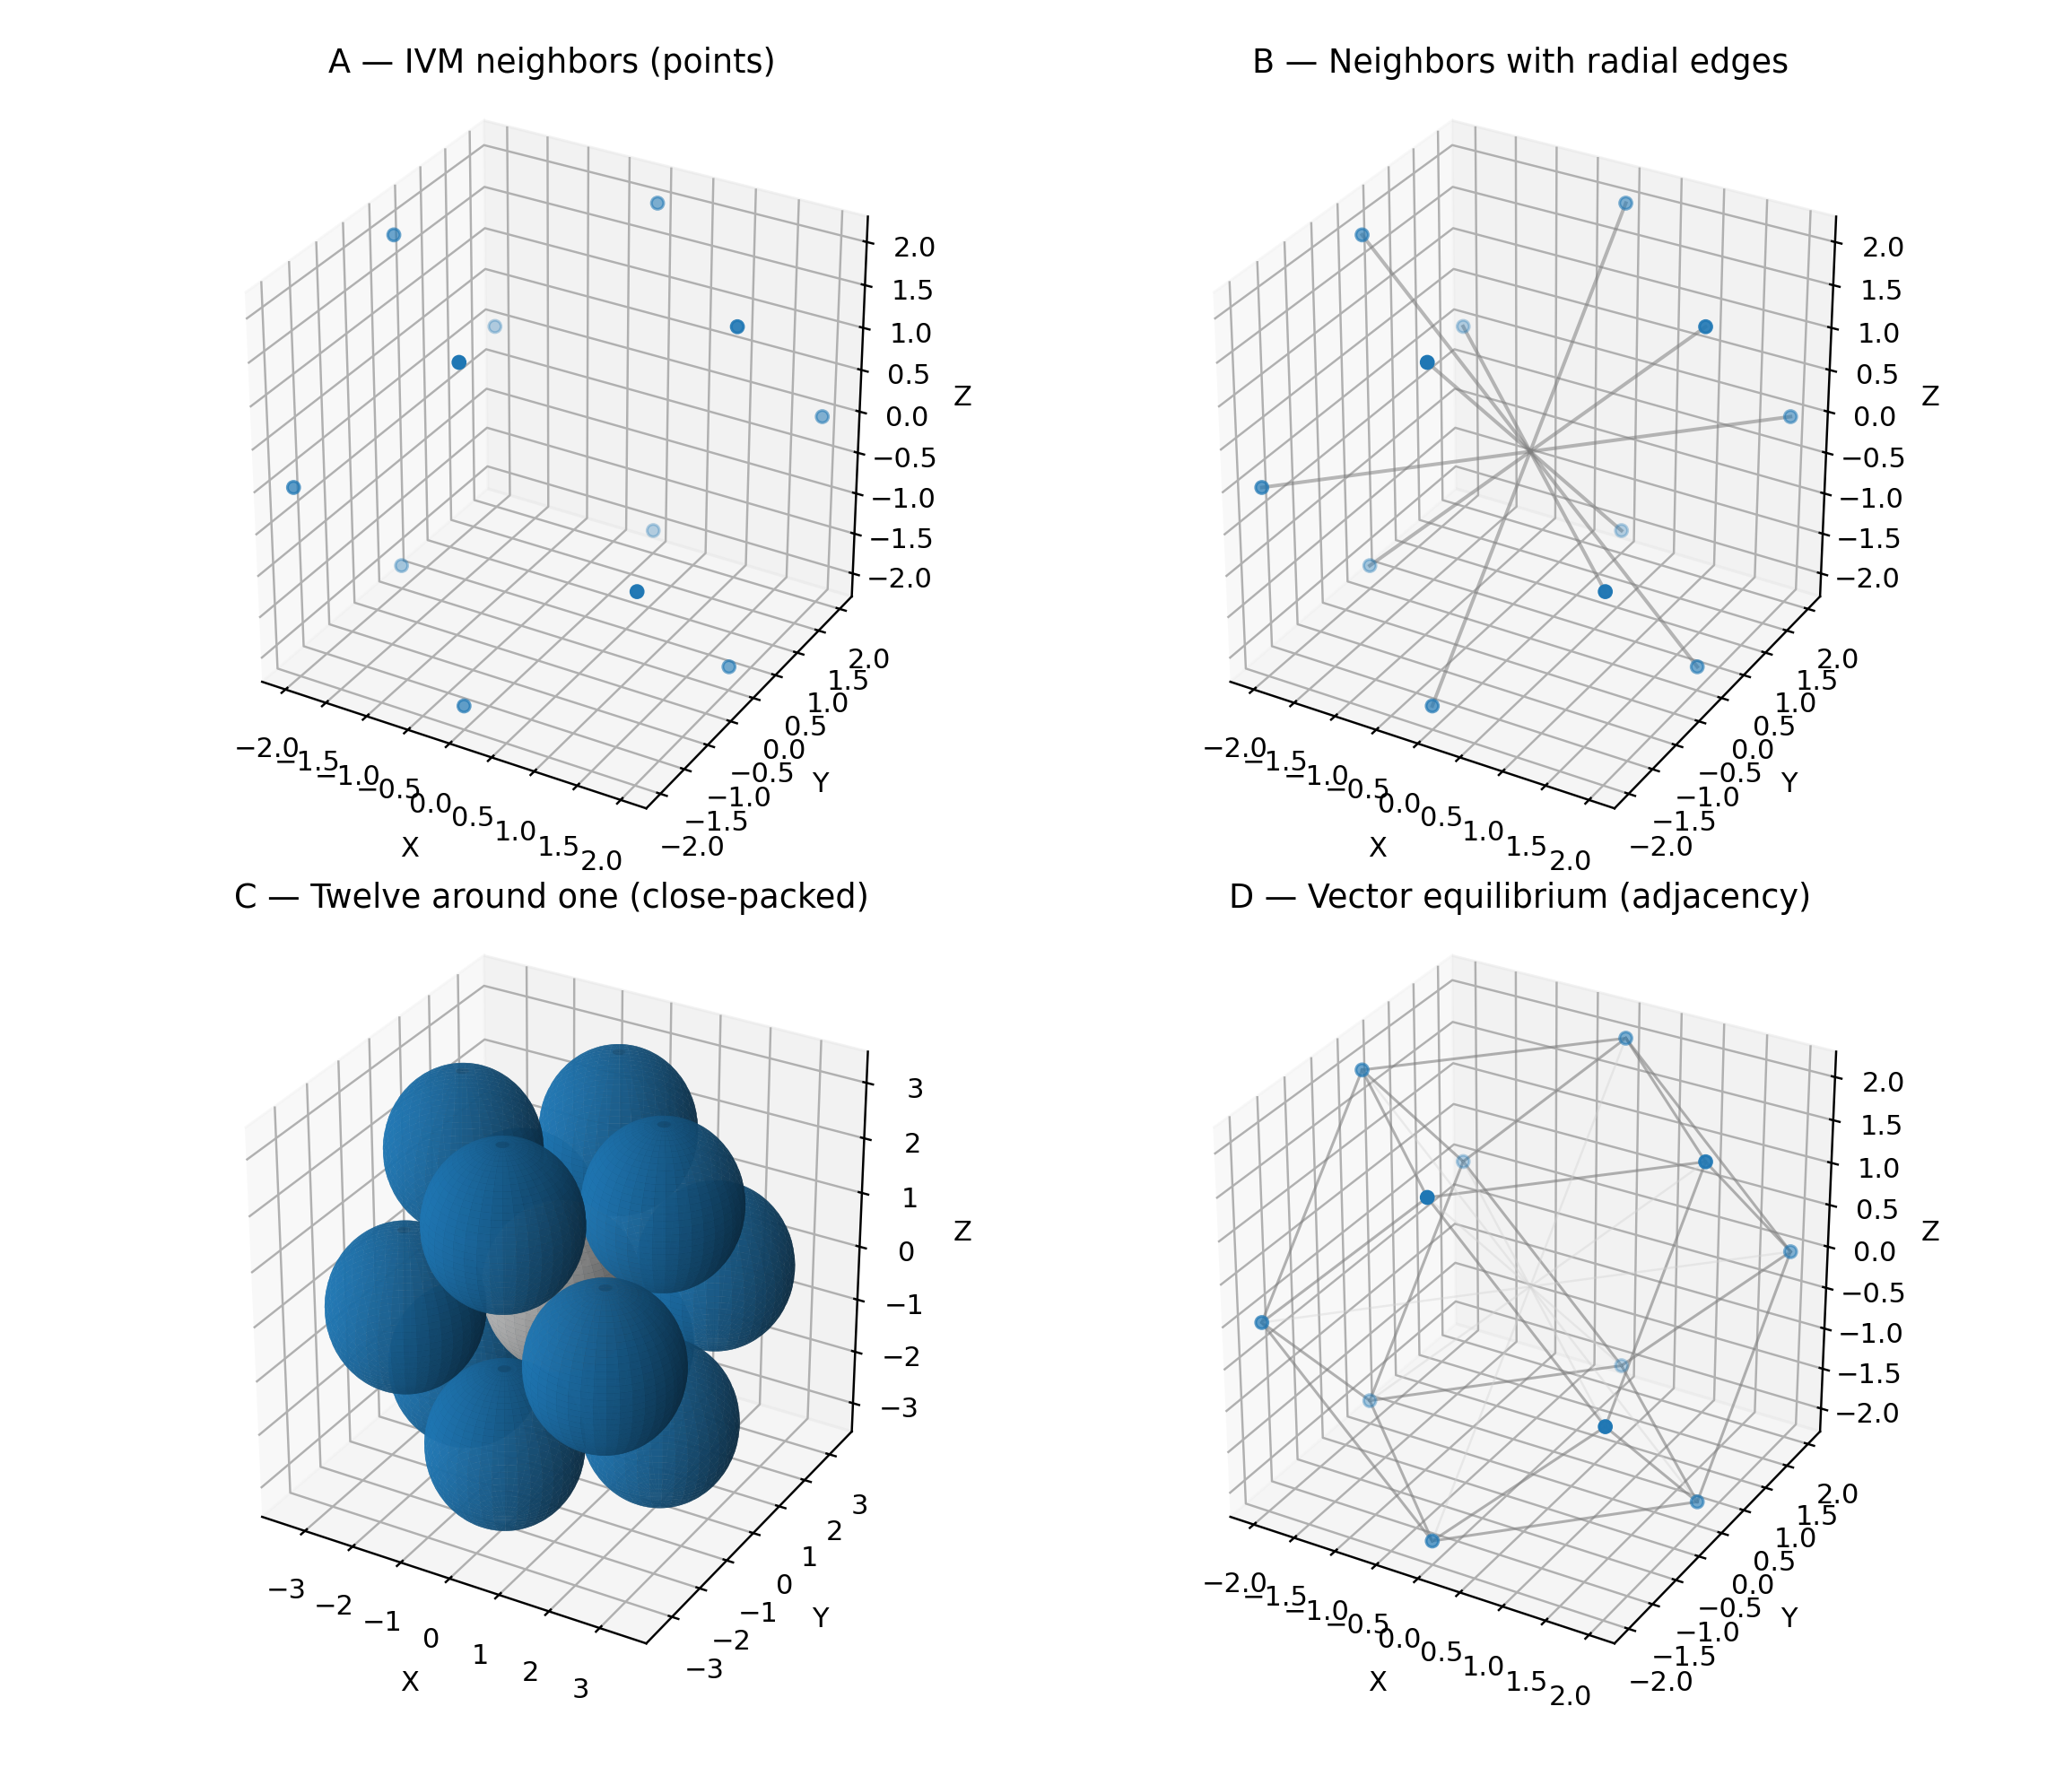
\includegraphics{../output/figures/ivm_neighbors_edges.png}
\caption{\textbf{IVM neighbors and coordination patterns (2×2 panel
layout)}. \textbf{Panel A}: The twelve nearest IVM neighbors plotted as
blue points in 3D space under the default embedding, showing the
positions corresponding to permutations of the Quadray integer
coordinates \{2,1,1,0\}. These points form the vertices of a
cuboctahedron (vector equilibrium) centered at the origin with uniform
radial distances. \textbf{Panel B}: The same neighbor points with radial
edges (light lines) connecting each neighbor to the central origin,
emphasizing the spoke-like radial symmetry and equal distances from
center to shell. \textbf{Panel C}: Twelve-around-one close-packed
spheres configuration where each neighbor position hosts a sphere with
radius chosen so neighboring spheres kiss along cuboctahedron edges,
illustrating the fundamental CCP/FCC/IVM correspondence. The central
gray sphere represents the ``one'' in Fuller's ``twelve around one''
motif. \textbf{Panel D}: Adjacency graph showing strut connections
(solid lines) between touching neighbor spheres, revealing the
cuboctahedron's edge structure, plus light radial cables to the origin
representing a stylized tensegrity interpretation of the vector
equilibrium geometry.}
\end{figure}

\begin{figure}
\centering
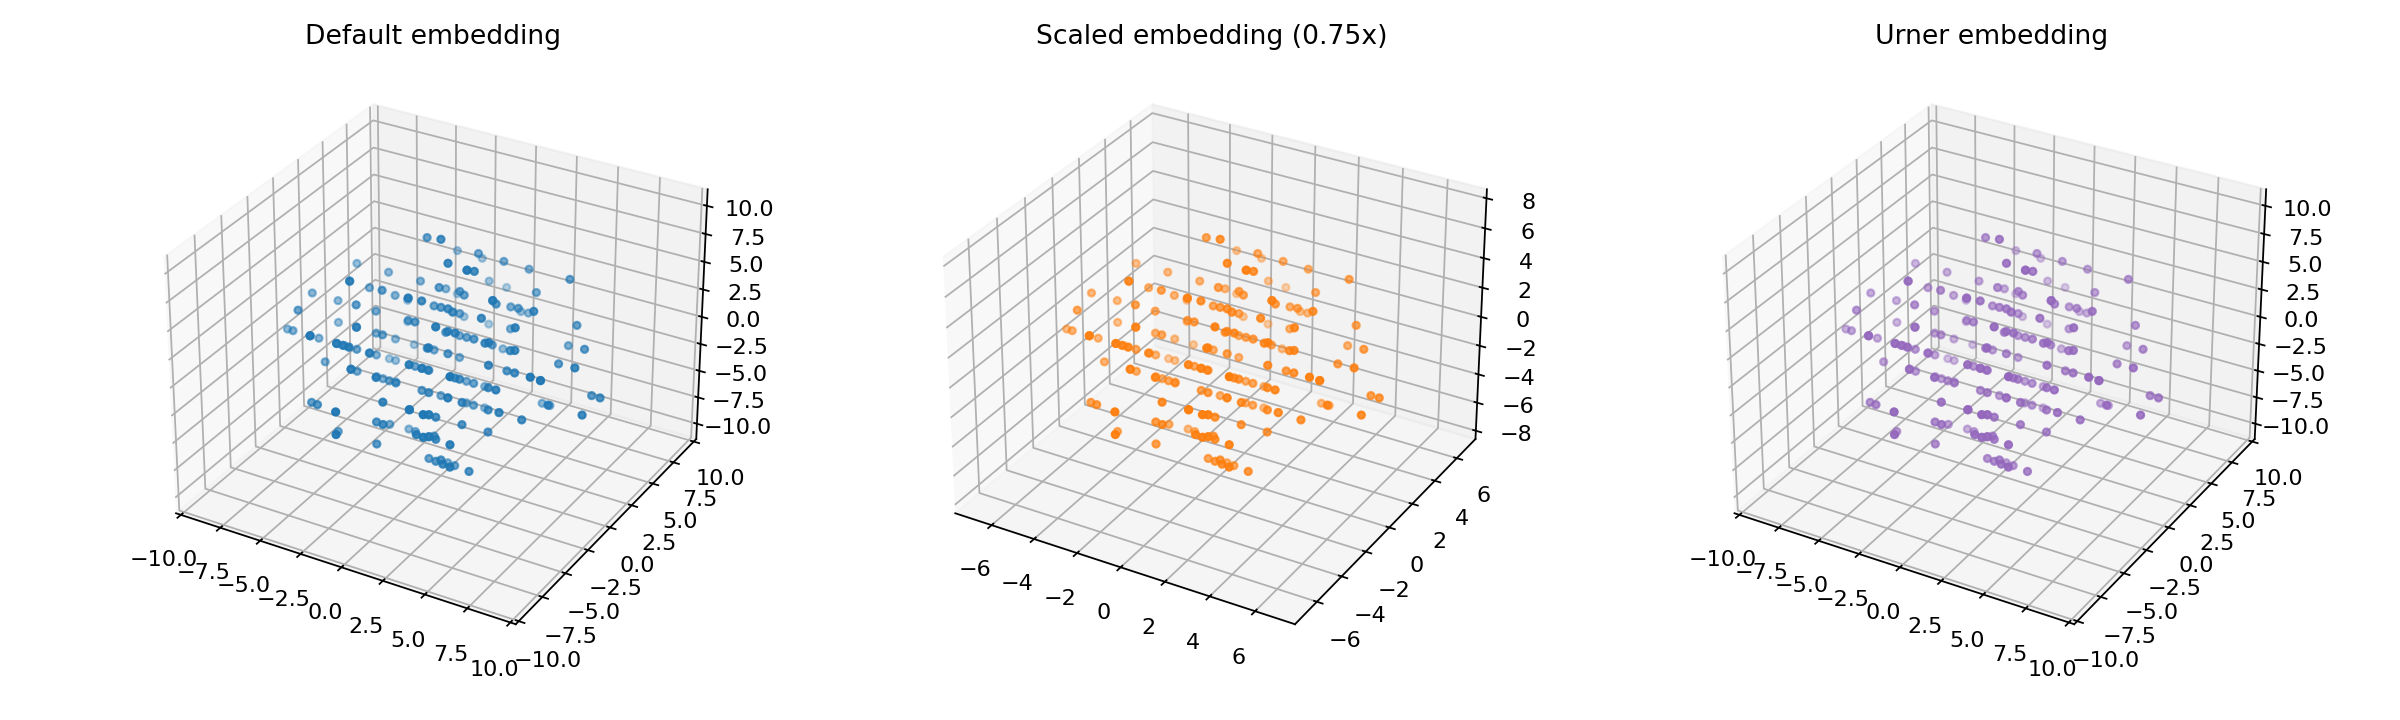
\includegraphics{../output/figures/quadray_clouds.png}
\caption{\textbf{Random Quadray point clouds under different embeddings
(3-panel comparison)}. Each panel shows 200 randomly sampled integer
Quadray coordinates with components in \{0,1,2,3,4,5\} projected to 3D
space using different embedding matrices. \textbf{Left panel (Default
embedding)}: Points (blue) under the default symmetric embedding matrix
showing the natural tetrahedral-symmetric distribution of normalized
Quadrays in 3D space. \textbf{Center panel (Scaled embedding, 0.75×)}:
The same Quadray points (orange) under a uniformly scaled version of the
default embedding, demonstrating how the point cloud structure scales
proportionally while preserving relative geometries. \textbf{Right panel
(Urner embedding)}: The same points (purple) projected through the
canonical Urner embedding matrix, illustrating how different linear
mappings from Fuller.4D to Coxeter.4D (3D slice) affect the spatial
distribution while preserving the underlying discrete lattice
relationships. This comparison demonstrates the flexibility in choosing
embeddings for visualization and analysis while maintaining the
fundamental Quadray coordinate relationships.}
\end{figure}

In the previous figure, we show the twelve nearest IVM neighbors with
coordination patterns and vector equilibrium geometry; the current
figure illustrates random Quadray clouds under several embeddings.

\textbf{Vector equilibrium (cuboctahedron)}: The shell formed by the 12
nearest IVM neighbors is the cuboctahedron, also called the vector
equilibrium in synergetics. All 12 vertices are equidistant from the
origin with equal edge lengths, modeling a balanced local packing. This
geometry underlies the ``twelve around one'' close-packing motif and
appears in tensegrity discussions as a canonical balanced structure. See
background:
\href{https://en.wikipedia.org/wiki/Cuboctahedron}{Cuboctahedron (vector
equilibrium)} and synergetics references. Computational demonstrations
include related visualizations in the 4dsolutions ecosystem. See the
\href{07_resources.md}{Resources} section for comprehensive details.

\hypertarget{clarifying-remarks}{%
\subsubsection{Clarifying remarks}\label{clarifying-remarks}}

``A time machine is not a tesseract.''
\href{https://groups.io/g/synergeo/topic/my_take_on_close_pack/114531919}{KU
on synergeo} The tesseract is a Euclidean 4D object (Coxeter.4D), while
Minkowski spacetime (Einstein.4D) is indefinite and not Euclidean;
conflating the two leads to category errors. Fuller.4D, in turn, is a
tetrahedral, mereological framing of ordinary space emphasizing
shape/angle relations and IVM quantization. Each namespace carries
distinct assumptions and should be used accordingly in analysis.

\hypertarget{practical-usage-guide}{%
\subsection{Practical usage guide}\label{practical-usage-guide}}

\begin{itemize}
\tightlist
\item
  Use \textbf{Fuller.4D} when working with Quadrays, integer
  tetravolumes, and IVM neighbors (native lattice calculations).
\item
  Use \textbf{Coxeter.4D} for Euclidean length-based formulas,
  higher-dimensional polytopes, or comparisons in E⁴ (including
  Cayley--Menger).
\item
  Use \textbf{Einstein.4D} as a metric analogy when discussing geodesics
  or time-evolution; do not mix with synergetic unit conventions.
\end{itemize}

\end{document}
